% !TEX TS-program = pdflatex
\documentclass[11pt]{article}

% -------------------- Packages --------------------
\usepackage[a4paper,margin=1in]{geometry}
\usepackage{amsmath,amssymb}
\usepackage[T1]{fontenc}
\usepackage{lmodern}
\usepackage{xcolor}
\usepackage{tcolorbox}
\tcbuselibrary{skins,breakable}
\usepackage{enumitem}
\usepackage{hyperref}
\usepackage{tikz}
\usetikzlibrary{angles,quotes,calc}

\pagestyle{empty}

% -------------------- Dark Theme Colors --------------------
\definecolor{bg}{HTML}{000000}
\definecolor{pairbg}{HTML}{121212}
\definecolor{solbg}{HTML}{0A0A0A}
\definecolor{border}{HTML}{2A2A2A}
\definecolor{text}{HTML}{FFFFFF}
\definecolor{muted}{HTML}{C9CDD3}
\definecolor{gold}{HTML}{FFD700}
\definecolor{green}{HTML}{4ADE80}
\definecolor{cyan}{HTML}{38BDF8}

\pagecolor{bg}
\color{text}

\hypersetup{
  colorlinks=true,
  linkcolor=cyan,
  urlcolor=cyan
}

\setlength{\parindent}{0pt}
\setlength{\parskip}{10pt}

% helps prevent text going out of the box
\setlength{\emergencystretch}{3em}
\sloppy

\setlist[itemize]{left=1.4em,itemsep=6pt,topsep=6pt}
\setlist[enumerate]{left=1.6em,itemsep=4pt,topsep=4pt}

% -------------------- tcolorbox Base --------------------
\tcbset{
  enhanced,
  breakable,
  arc=12pt,
  boxrule=0.8pt,
  left=16pt,right=16pt,top=12pt,bottom=12pt,
  before upper=\raggedright
}

\newtcolorbox{QAPair}[1]{%
  colback=pairbg,
  colbacklower=solbg,
  colframe=border,
  coltext=text,
  title=\textcolor{gold}{\bfseries #1},
  fonttitle=\bfseries,
  coltitle=text,
  segmentation style={draw=border, dashed, line width=0.6pt},
}

\newtcolorbox{QuickBox}{%
  colback=pairbg,
  colframe=cyan,
  coltext=text,
  fontupper=\color{text},
  borderline north={4pt}{0pt}{cyan},
  arc=14pt,
  boxrule=0.8pt
}

% Helper for step headings
\newcommand{\Step}[1]{\textcolor{muted}{\textbf{Step #1:}}}

% -------------------- TikZ styles --------------------
\tikzset{
  tri/.style={line width=0.9pt, draw=muted},
  lab/.style={text=text, font=\small},
  mlabel/.style={text=muted, font=\small},
}

% ============================================================
\begin{document}

\begin{center}
{\LARGE\bfseries \textcolor{gold}{Exercise 6.5 --- Solutions}}\\[-2pt]
\end{center}

\begin{QuickBox}
{\color{cyan}\bfseries Quick formulas (useful)}\par\medskip
\begin{itemize}
\item \textbf{Right triangle:} $\tan\theta=\dfrac{\text{opposite}}{\text{adjacent}},\;\;
\sin\theta=\dfrac{\text{opposite}}{\text{hypotenuse}},\;\;
\cos\theta=\dfrac{\text{adjacent}}{\text{hypotenuse}}$.
\item \textbf{Angles:} angle of depression = angle of elevation (alternate interior angles).
\item \textbf{Special values:} $\tan 30^\circ=\dfrac{1}{\sqrt3},\;\tan 45^\circ=1,\;\tan 60^\circ=\sqrt3$;\;\;
$\sin 30^\circ=\dfrac12$.
\item \textbf{Equilateral triangle height:} $h=\dfrac{\sqrt3}{2}a$.
\end{itemize}
\end{QuickBox}

% ============================================================
% Q1
\begin{QAPair}{Question 1}
\textcolor{gold}{\bfseries Question:} From a point at a distance of $20$ m from a tree, angle of elevation of top is $30^\circ$. Find height of the tree.\\
\tcblower
\textcolor{green}{\bfseries Diagram:}
\begin{center}
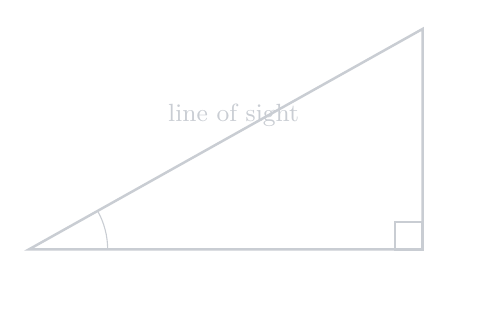
\begin{tikzpicture}[scale=1.0]
  \coordinate (A) at (0,0);   % observer
  \coordinate (B) at (5,0);   % tree base
  \coordinate (C) at (5,2.8); % tree top
  \draw[tri] (A)--(B)--(C)--cycle;
  \draw[tri] (B) rectangle ++(-0.35,0.35);

  \pic [draw=muted, angle radius=10mm, angle eccentricity=1.25] {angle = B--A--C};
  \node[lab] at (1.2,0.35) {$30^\circ$};

  \node[lab] at (2.5,-0.35) {$20$ m};
  \node[lab] at (5.35,1.4) {$h$};
  \node[mlabel] at (2.6,1.7) {line of sight};
\end{tikzpicture}
\end{center}

\textcolor{green}{\bfseries Answer:}
\[
\begin{aligned}
\Step{1}\;& \tan 30^\circ=\frac{h}{20}.\\
\Step{2}\;& h=20\tan 30^\circ=20\cdot\frac{1}{\sqrt3}=\frac{20}{\sqrt3}
=\frac{20\sqrt3}{3}\text{ m}.
\end{aligned}
\]
\end{QAPair}

% ============================================================
% Q2
\begin{QAPair}{Question 2}
\textcolor{gold}{\bfseries Question:} A pole is $10$ m high and its shadow is $10\sqrt3$ m. Find the angle of elevation of the sun.\\
\tcblower
\textcolor{green}{\bfseries Diagram:}
\begin{center}
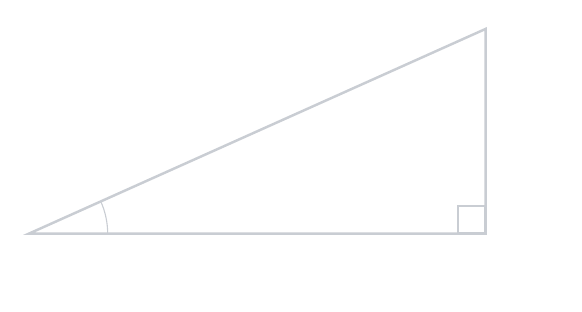
\begin{tikzpicture}[scale=1.0]
  \coordinate (A) at (0,0);     % shadow end
  \coordinate (B) at (5.8,0);   % pole base
  \coordinate (C) at (5.8,2.6); % pole top
  \draw[tri] (A)--(B)--(C)--cycle;
  \draw[tri] (B) rectangle ++(-0.35,0.35);

  \pic [draw=muted, angle radius=10mm, angle eccentricity=1.25] {angle = B--A--C};
  \node[lab] at (1.2,0.35) {$\theta$};

  \node[lab] at (2.9,-0.35) {$10\sqrt3$ m};
  \node[lab] at (6.2,1.3) {$10$ m};
\end{tikzpicture}
\end{center}

\textcolor{green}{\bfseries Answer:}
\[
\begin{aligned}
\Step{1}\;& \tan\theta=\frac{\text{height}}{\text{shadow}}
=\frac{10}{10\sqrt3}=\frac{1}{\sqrt3}.\\
\Step{2}\;& \tan\theta=\tan 30^\circ \Rightarrow \theta=30^\circ.
\end{aligned}
\]
\end{QAPair}

% ============================================================
% Q3
\begin{QAPair}{Question 3}
\textcolor{gold}{\bfseries Question:} A window is an equilateral triangle of side $1.6$ m. Find height of the window.\\
\tcblower
\textcolor{green}{\bfseries Diagram:}
\begin{center}
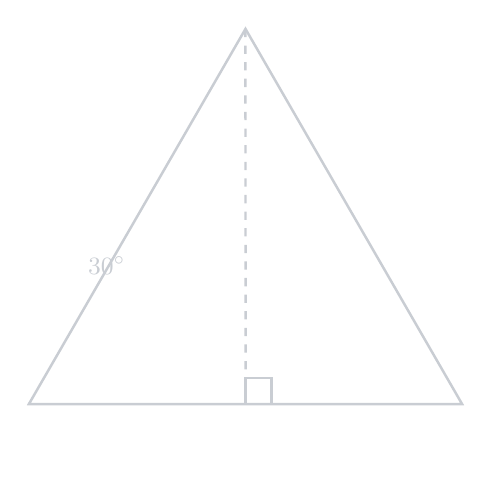
\begin{tikzpicture}[scale=1.1]
  \coordinate (A) at (0,0);
  \coordinate (B) at (5,0);
  \coordinate (C) at (2.5,4.33); % approx equilateral
  \draw[tri] (A)--(B)--(C)--cycle;

  \coordinate (D) at ($(A)!0.5!(B)$);
  \draw[tri, dashed] (C)--(D);
  \draw[tri] (D) rectangle ++(0.3,0.3);

  \node[lab] at (2.5,-0.35) {$1.6$ m};
  \node[lab] at (2.85,2.0) {$h$};
  \node[mlabel] at (0.9,1.6) {$30^\circ$};
\end{tikzpicture}
\end{center}

\textcolor{green}{\bfseries Answer:}
\[
\begin{aligned}
\Step{1}\;& \text{In an equilateral triangle, } h=\frac{\sqrt3}{2}a.\\
\Step{2}\;& h=\frac{\sqrt3}{2}\cdot 1.6=0.8\sqrt3\text{ m}\approx 1.386\text{ m}.
\end{aligned}
\]
\end{QAPair}

% ============================================================
% Q4
\begin{QAPair}{Question 4}
\textcolor{gold}{\bfseries Question:} Height of a slide is $5$ m. From the top, the angle of depression of the bottom is $30^\circ$. Find the length of the slide.\\
\tcblower
\textcolor{green}{\bfseries Diagram:}
\begin{center}
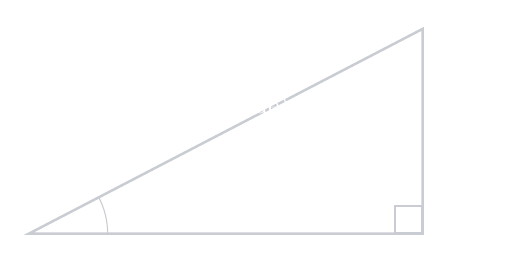
\begin{tikzpicture}[scale=1.0]
  \coordinate (B) at (0,0);   % bottom
  \coordinate (A) at (5,0);   % foot below top
  \coordinate (C) at (5,2.6); % top
  \draw[tri] (B)--(A)--(C)--cycle;
  \draw[tri] (A) rectangle ++(-0.35,0.35);

  \pic [draw=muted, angle radius=10mm, angle eccentricity=1.25] {angle = A--B--C};
  \node[lab] at (1.2,0.35) {$30^\circ$};

  \node[lab] at (5.35,1.3) {$5$ m};
  \node[lab] at (2.7,1.6) {$L$ (slide)};
\end{tikzpicture}
\end{center}

\textcolor{green}{\bfseries Answer:}
\[
\begin{aligned}
\Step{1}\;& \text{Angle of depression }=30^\circ \Rightarrow \text{angle of elevation }=30^\circ.\\
\Step{2}\;& \sin 30^\circ=\frac{\text{opposite}}{\text{hypotenuse}}=\frac{5}{L}.\\
\Step{3}\;& \frac12=\frac{5}{L}\Rightarrow L=10\text{ m}.
\end{aligned}
\]
\end{QAPair}

% ============================================================
% Q5
\begin{QAPair}{Question 5}
\textcolor{gold}{\bfseries Question:} Two pillars of equal height stand on either side of a roadway $120$ m wide. From a point between them, angles of elevation are $60^\circ$ and $30^\circ$. Find the height of each pillar and the position of the point.\\
\tcblower
\textcolor{green}{\bfseries Diagram:}
\begin{center}
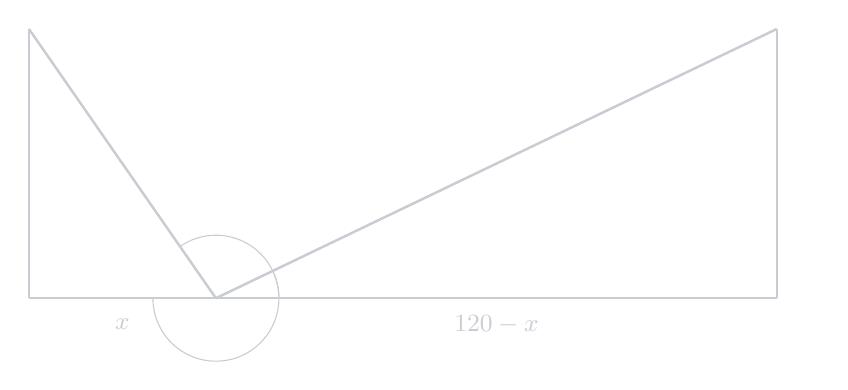
\begin{tikzpicture}[scale=0.95]
  \coordinate (L) at (0,0);     % left pillar base
  \coordinate (R) at (10,0);    % right pillar base
  \coordinate (P) at (2.5,0);   % observation point
  \coordinate (LT) at (0,3.6);  % left top
  \coordinate (RT) at (10,3.6); % right top

  \draw[tri] (L)--(R);
  \draw[tri] (L)--(LT);
  \draw[tri] (R)--(RT);
  \draw[tri] (P)--(LT);
  \draw[tri] (P)--(RT);

  \node[lab] at (5,-0.4) {$120$ m};
  \node[lab] at (0.35,1.8) {$h$};
  \node[lab] at (10.35,1.8) {$h$};

  \pic [draw=muted, angle radius=8mm, angle eccentricity=1.25] {angle = L--P--LT};
  \node[lab] at (1.5,0.45) {$60^\circ$};

  \pic [draw=muted, angle radius=8mm, angle eccentricity=1.25] {angle = R--P--RT};
  \node[lab] at (3.9,0.35) {$30^\circ$};

  \node[mlabel] at (1.25,-0.35) {$x$};
  \node[mlabel] at (6.25,-0.35) {$120-x$};
\end{tikzpicture}
\end{center}

\textcolor{green}{\bfseries Answer:}
Let distance from point to the pillar with $60^\circ$ be $x$ m, so the other distance is $(120-x)$ m.
\[
\begin{aligned}
\Step{1}\;& \tan 60^\circ=\frac{h}{x}\Rightarrow h=x\sqrt3.\\
\Step{2}\;& \tan 30^\circ=\frac{h}{120-x}\Rightarrow h=\frac{120-x}{\sqrt3}.\\
\Step{3}\;& x\sqrt3=\frac{120-x}{\sqrt3}\Rightarrow 3x=120-x\Rightarrow 4x=120\Rightarrow x=30.\\
\Step{4}\;& h=x\sqrt3=30\sqrt3\text{ m}.\\
\Step{5}\;& \text{Position: }30\text{ m from the }60^\circ\text{ pillar and }90\text{ m from the other.}
\end{aligned}
\]
\end{QAPair}

% ============================================================
% Q6
\begin{QAPair}{Question 6}
\textcolor{gold}{\bfseries Question:} From the top of a $120$ m tower, angles of depression of two boats on the same side are $60^\circ$ and $45^\circ$. Find the distance between the boats.\\
\tcblower
\textcolor{green}{\bfseries Diagram:}
\begin{center}
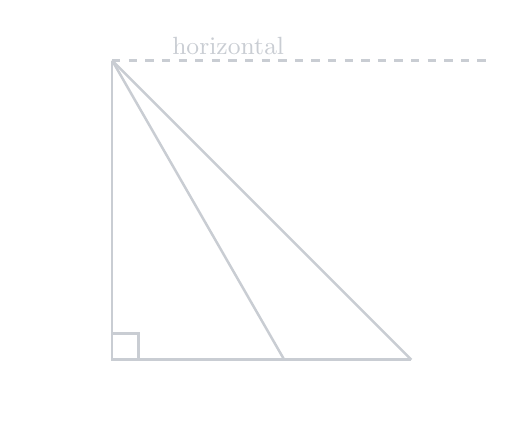
\begin{tikzpicture}[scale=0.95]
  \coordinate (B) at (0,0);    % tower base
  \coordinate (T) at (0,4);    % tower top
  \coordinate (P1) at (2.3,0); % nearer boat (60)
  \coordinate (P2) at (4.0,0); % farther boat (45)

  \draw[tri] (B)--(T);
  \draw[tri] (B)--(P2);
  \draw[tri] (T)--(P1);
  \draw[tri] (T)--(P2);

  \draw[tri] (B) rectangle ++(0.35,0.35);

  \node[lab] at (-0.55,2.0) {$120$ m};

  \draw[tri, dashed] (T)--++(5,0);
  \node[mlabel] at (1.55,4.2) {horizontal};

  \node[lab] at (2.2,-0.35) {$d_1$};
  \node[lab] at (4.0,-0.35) {$d_2$};

  \node[lab] at (1.2,3.25) {$60^\circ$};
  \node[lab] at (2.0,2.7) {$45^\circ$};
\end{tikzpicture}
\end{center}

\textcolor{green}{\bfseries Answer:}
\[
\begin{aligned}
\Step{1}\;& \text{Angle of depression equals angle of elevation, so use }60^\circ,45^\circ\text{ at the boats.}\\
\Step{2}\;& d_1=\frac{120}{\tan 60^\circ}=\frac{120}{\sqrt3}=40\sqrt3\text{ m}.\\
\Step{3}\;& d_2=\frac{120}{\tan 45^\circ}=120\text{ m}.\\
\Step{4}\;& \text{Distance between boats }=d_2-d_1=120-40\sqrt3\text{ m}\approx 50.72\text{ m}.
\end{aligned}
\]
\end{QAPair}

% ============================================================
% Q7
\begin{QAPair}{Question 7}
\textcolor{gold}{\bfseries Question:} Two men on opposite sides of a tree are in line with it. Angles of elevation of the top are $30^\circ$ and $60^\circ$. Height of the tree is $15$ m. Find distance between the men.\\
\tcblower
\textcolor{green}{\bfseries Diagram:}
\begin{center}
\begin{tikzpicture}[scale=0.95]
  \coordinate (O) at (0,0);      % tree base
  \coordinate (T) at (0,3.8);    % tree top
  \coordinate (A) at (-4.8,0);   % man 30
  \coordinate (B) at (2.8,0);    % man 60

  \draw[tri] (O)--(T);
  \draw[tri] (A)--(O)--(B);
  \draw[tri] (A)--(T);
  \draw[tri] (B)--(T);

  \node[lab] at (0.5,1.9) {$15$ m};
  \node[mlabel] at (-2.4,-0.35) {$y$};
  \node[mlabel] at (1.4,-0.35) {$x$};

  \node[lab] at (-3.6,0.45) {$30^\circ$};
  \node[lab] at (1.9,0.45) {$60^\circ$};
\end{tikzpicture}
\end{center}

\textcolor{green}{\bfseries Answer:}
Let distances of the men from the tree be $y$ (for $30^\circ$) and $x$ (for $60^\circ$).
\[
\begin{aligned}
\Step{1}\;& \tan 60^\circ=\frac{15}{x}\Rightarrow x=\frac{15}{\sqrt3}=5\sqrt3.\\
\Step{2}\;& \tan 30^\circ=\frac{15}{y}\Rightarrow y=15\sqrt3.\\
\Step{3}\;& \text{Distance between men }=x+y=5\sqrt3+15\sqrt3=20\sqrt3\text{ m}\approx 34.64\text{ m}.
\end{aligned}
\]
\end{QAPair}

% ============================================================
% Q8
\begin{QAPair}{Question 8}
\textcolor{gold}{\bfseries Question:} From the top of a $12$ m tree, the angles of elevation and depression of the top and bottom of a building are $30^\circ$ and $45^\circ$ respectively. Find the height of the building and the distance between the tree and the building.\\
\tcblower
\textcolor{green}{\bfseries Diagram:}
\begin{center}
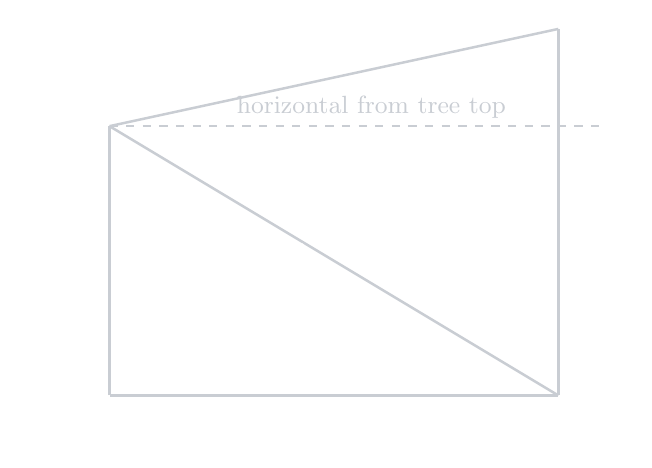
\begin{tikzpicture}[scale=0.95]
  \coordinate (TB) at (0,0);     % tree base
  \coordinate (TT) at (0,3.6);   % tree top
  \coordinate (BB) at (6,0);     % building base
  \coordinate (BT) at (6,4.9);   % building top (unknown)

  \draw[tri] (TB)--(TT);
  \draw[tri] (BB)--(BT);
  \draw[tri] (TB)--(BB);

  \draw[tri] (TT)--(BB);
  \draw[tri] (TT)--(BT);

  \draw[tri, dashed] (TT)--++(6.6,0);

  \node[lab] at (-0.6,1.8) {$12$ m};
  \node[lab] at (6.6,2.45) {$H$};

  \node[lab] at (3.0,-0.35) {$d$};

  \node[mlabel] at (3.5,3.85) {horizontal from tree top};

  \node[lab] at (2.0,3.2) {$30^\circ$};
  \node[lab] at (2.4,1.9) {$45^\circ$};
\end{tikzpicture}
\end{center}

\textcolor{green}{\bfseries Answer:}
Let the horizontal distance between tree and building be $d$ m, and building height be $H$ m.
\[
\begin{aligned}
\Step{1}\;& \text{Angle of depression to building bottom }=45^\circ.\\
& \tan 45^\circ=\frac{12}{d}\Rightarrow 1=\frac{12}{d}\Rightarrow d=12\text{ m}.\\
\Step{2}\;& \text{Angle of elevation to building top }=30^\circ.\\
& \tan 30^\circ=\frac{H-12}{d}=\frac{H-12}{12}=\frac{1}{\sqrt3}.\\
\Step{3}\;& H-12=\frac{12}{\sqrt3}=4\sqrt3 \Rightarrow H=12+4\sqrt3\text{ m}.\\
\Step{4}\;& \boxed{d=12\text{ m}},\qquad \boxed{H=12+4\sqrt3\text{ m}\approx 18.93\text{ m}}.
\end{aligned}
\]
\end{QAPair}

% ============================================================
% Q9
\begin{QAPair}{Question 9}
\textcolor{gold}{\bfseries Question:} From point $A$ on ground at distance $200$ m from a tower, angle of elevation of the top is $\alpha$. Another point $B$ is $80$ m nearer to the tower. Angle of elevation from $B$ is $\beta$. If $\tan\alpha=\dfrac{2}{5}$, find height of tower and value of $\beta$.\\
\tcblower
\textcolor{green}{\bfseries Diagram:}
\begin{center}
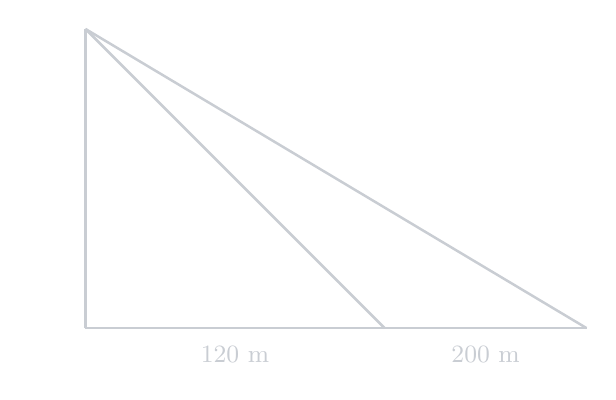
\begin{tikzpicture}[scale=0.95]
  \coordinate (O) at (0,0);     % tower base
  \coordinate (T) at (0,4);     % tower top
  \coordinate (B) at (4.0,0);   % nearer point (120)
  \coordinate (A) at (6.7,0);   % farther point (200)

  \draw[tri] (O)--(T);
  \draw[tri] (O)--(A);
  \draw[tri] (T)--(A);
  \draw[tri] (T)--(B);

  \node[lab] at (-0.55,2.0) {$h$};

  \node[mlabel] at (2.0,-0.35) {$120$ m};
  \node[mlabel] at (5.35,-0.35) {$200$ m};

  \node[lab] at (5.4,0.45) {$\alpha$};
  \node[lab] at (3.3,0.45) {$\beta$};
\end{tikzpicture}
\end{center}

\textcolor{green}{\bfseries Answer:}
\[
\begin{aligned}
\Step{1}\;& \tan\alpha=\frac{h}{200}=\frac{2}{5}\Rightarrow h=200\cdot\frac{2}{5}=80\text{ m}.\\
\Step{2}\;& \text{Point }B\text{ is }80\text{ m nearer, so distance from tower }=200-80=120\text{ m}.\\
\Step{3}\;& \tan\beta=\frac{h}{120}=\frac{80}{120}=\frac{2}{3}.\\
\Step{4}\;& \boxed{h=80\text{ m}},\qquad \boxed{\beta=\tan^{-1}\!\left(\frac{2}{3}\right)\approx 33.69^\circ}.
\end{aligned}
\]
\end{QAPair}

% ============================================================
% Q10
\begin{QAPair}{Question 10}
\textcolor{gold}{\bfseries Question:} A boat moves away from a lighthouse $206.6$ m high. It takes $120$ s for the angle of elevation of the top to change from $60^\circ$ to $45^\circ$. Find the speed of the boat.\\
\tcblower
\textcolor{green}{\bfseries Diagram:}
\begin{center}
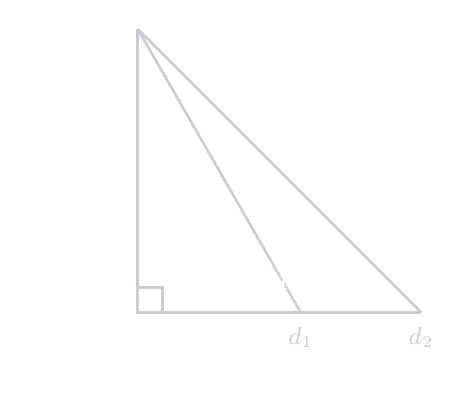
\begin{tikzpicture}[scale=0.9]
  \coordinate (O) at (0,0);      % lighthouse base
  \coordinate (T) at (0,4.0);    % lighthouse top
  \coordinate (P1) at (2.3,0);   % boat position 1 (60)
  \coordinate (P2) at (4.0,0);   % boat position 2 (45)

  \draw[tri] (O)--(T);
  \draw[tri] (O)--(P2);
  \draw[tri] (T)--(P1);
  \draw[tri] (T)--(P2);
  \draw[tri] (O) rectangle ++(0.35,0.35);

  \node[lab] at (-0.8,2.0) {$206.6$ m};

  \node[lab] at (1.3,0.45) {$60^\circ$};
  \node[lab] at (2.2,0.45) {$45^\circ$};

  \node[mlabel] at (2.3,-0.35) {$d_1$};
  \node[mlabel] at (4.0,-0.35) {$d_2$};

  \node[lab] at (3.15,-0.75) {$\Delta d=d_2-d_1$};
\end{tikzpicture}
\end{center}

\textcolor{green}{\bfseries Answer:}
Let lighthouse height $h=206.6$ m. If the angles of elevation are $60^\circ$ then $45^\circ$, the horizontal distances are:
\[
\begin{aligned}
\Step{1}\;& d_1=\frac{h}{\tan 60^\circ}=\frac{206.6}{\sqrt3}\text{ m},\qquad
d_2=\frac{h}{\tan 45^\circ}=206.6\text{ m}.\\
\Step{2}\;& \Delta d=d_2-d_1
=206.6-\frac{206.6}{\sqrt3}\text{ m}.\\
\Step{3}\;& \text{Speed }v=\frac{\Delta d}{120}
=\frac{206.6-\frac{206.6}{\sqrt3}}{120}\text{ m/s}.
\end{aligned}
\]

Numerically,
\[
\frac{206.6}{\sqrt3}\approx 119.25,\quad
\Delta d\approx 87.35\text{ m},\quad
v\approx \frac{87.35}{120}\approx 0.728\text{ m/s}\approx 2.62\text{ km/h}.
\]
\end{QAPair}

\end{document}
